\clearpage
\section{Kódování snižující nadbytečnost}
\subsection{ Vysvětlete základní princip snižování nadbytečnosti}
Při realizaci přizpůsobení zdroje na kanál pomocí rovnoměrného kódování dochází k vyoké nadbytečnosti -> menší účinnost.
Řešením tohoto problému je využití nerovnoměrného kódování, které znakům s častějším výskytem přiřazuje značku s menším počtem bitů -> zkrácení doby přenosu oproti rovnoměrnému kódování -> zkrácení střední délky značky a zvýšení průměrné entropie na jeden bit zprávy.

\subsection{Co je to prefixový kód? Popište způsob dekódování.}
\begin{itemize}
    \item Prefixový kód je \textbf{nerovnoměrný kód}, pro nější platí, že žádná značka není prefixem jiné značky.
    \item Kódování se nazývá prefixovo, pokud je \textit{prosté}, tj. je realizováno prostým přiřazením a žádná značky není prefixem jiné značky.
    \item \textbf{Pokud je kód prefixový, je jednoznačně dekódovatelný}

\end{itemize}
\textbf{Dekódování}
\begin{itemize}
    \item Po přijmutí značky v ní najdeme nejmenší počet signálových prvků (zleva), které tvoří některou z užívaných značek.
    Tím považujeme první zprávu za dekódovanou a tyto prvky "umažeme".
    Poté opět hledáme nejmenší počet signálových prvků (opět zleva), které tvoří nekterou z užívaných značek a získáváme druhou zprávu \dots
\end{itemize}

\subsection{Co specifikuje Kraft-McMilanovo číslo, Kraftova nerovnost a McMilanova věta}
Mějme kód definovám předpisem S->X, poté \textbf{KraftMilanovo číslo} specifikuje
\begin{itemize}
    \item m$_i$ - počet symbolů v S, které jsou kódovány řetěžci dělky \emph{i} z množiny X.
    \item M - maximální délka kódovaného slova užívající F prvkového tělesa
    $$K = \sum_{i=1}^M \frac{m_i}{F^i}= \frac{m_1}{F^1} + \frac{m_2}{F^2} +\dots +\frac{m_M}{F^M}$$
\end{itemize}
\textbf{McMilanova věta}
\begin{itemize}
    \item Pro jednoznačně dekódovatelný kód platí Kraftova nerovnost $K \leqq 1$
    \item Věta však neplatí obráceně.
    I pří K < 1 nemusí být kód jednoznačně dekódovatelný.
    Z McMilanovy věty vychází
    \begin{itemize}
        \item K < 1 - kód má nadbytečnost a může být jednoznačně identifikován
        \item K = 1 - jedná s o tzv. kompletní kód a může být jednoznačně identifikován.
        \item K > 1 - kód není jednoznačně dekódovatelný
    \end{itemize}
\end{itemize}
\subsection{Uvěďte příklady algoritmů pro bezztrátovou kompresi}
\begin{enumerate}
    \item Aritmetické kódování (délka značek podle jejich pravděpodobností)
    \item Kódování s dynamickým slovníkem (LZW algoritmus)
\end{enumerate}

\subsection{Co je optimální kód, pomocí které veličiny můžeme tyto kódy porovnávat}
Nalezení optimálního kódu vede  na optimalizační problém, což je hledání minimální střední délky značky změnou délek jednotlivých $n_1, n_2, n_3 \dots n_n$, pro známí soubor pravděpodobností $p_1, p_2, \dots p_n$ pří splnění Kraftovy nerovnosti
$$\Bar{n}_{opt} = min \{\Bar{n}\},$$ kde
$$\Bar{n}=\sum_{i=1}^q p_i*n_i$$ a 
$$K\leqq1$$
Tedy hledáme takové délky $n_1=? \dots n_n=?$ pro zadané $p_1,p_2\dots p_n$ pro které je střední délka značky minimální, je splněna Kraftova nerovnost a kód je jednoznačně dekódovatelný, tj. prefixový.

Kódy lze porovnávat podle $\Bar{n}_{opt}$ (?)

\subsection{vysvětlete princip Huffmanova kódu}
Kód je založen na Huffmanově pravidle, které umožňuje navržení optimálního kódu.

\begin{enumerate}
    \item V množině symoblů primárního zdroje vyhledáme dva symboly s nejmenší pravděpodobností a sloučíme je.
    \item U původních symbolů si poznačíme 0 a 1
    \item Kroky 1) a 2) opakujeme dokud nevytvoříme zdroj s pouze jedním prvkem
    \item Kódová slova vytváříme zpětným procházením vytvořeného stromu a zapisováním si 0 a 1.
\end{enumerate}

\subsection{Vysvětlete princip a důvod použití kódování bloků dat}
\begin{enumerate}
    \item Může nastat situace, že množina prvků zdrojové abecedy S je menší než množina prvků pomocného zdroje 
    X->q->F, nebo je počet prvků zdrojové abecedy moc malý pro provedení efektivní datové komprese. 
    Příkladem může být černobílý obrázek, který je složený ze 2 prvků zdrojové abecedy černého a bílého bodu.
    V takovém případě můžeme využít sloučení více prvků primární abecedy a vytvořit tak novou sadu s vyšším počtem prvků.
    \item Chceme snižovat redundanci a zvyšovat entropii. Je vhodné kódovat často opakované kódy kratší značkou, 
    hledáme vhodné kódování.
\end{enumerate}

\subsection{Vysvětlete princip Aritmetického kódování a porovnejte s Huffmanovým kódem}
\begin{itemize}
    \item \textbf{Aritmetické kódování} realizuje návrh značky pro každý symbol primární abecedy individuálně, což umožňuje efektivně modifikovat kód v případě změny v jejím výskytu.
    \item V tomto kódování se využívá vyjádření reálného čísla v rozsahu (0,1) v binárním vyjádření ve tvaru
    $$0.x_1x_2x_3\dots x_n=\frac{x_1}{2}+\frac{x_2}{2^2}+\dots+\frac{x_n}{2^n}$$
    \item Např.:
    $$0.1101010=\frac{1}{2}+\frac{1}{4}+\frac{1}{16}+\frac{1}{64}=\frac{32+16+4+1}{64}=\frac{53}{64}=0,828125$$
    \item Postup:
    \begin{enumerate}
        \item Pro každý prvek spočítáme $a$, kde $a$ je kumulativní pravděpodobnost předchozích prvků.
        \item  Pro každý prvek i s pravděpodobnost pi určíme n tak, aby bylo nejbližším vyšším celým číslem 
        splňujícím nerovnost $n \geq 1 - log_2 p_i$.
        \item Určíme celé číslo c, pro něž platí: $c - 1 \leq 2^n a_i < c $
        \item $c$ převedeme na kódové slovo
    \end{enumerate}
    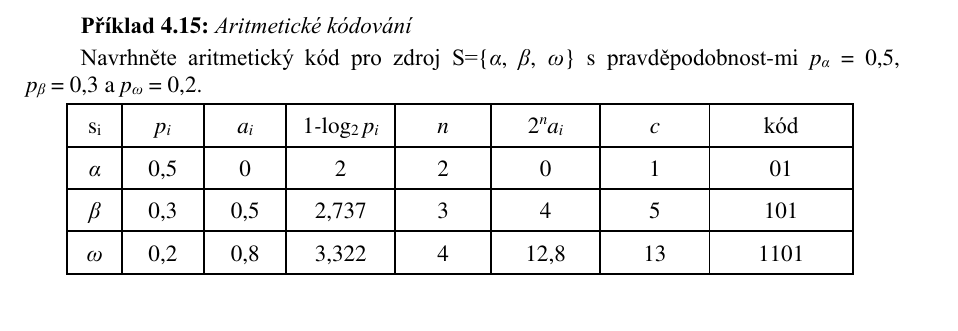
\includegraphics[width=15.5cm]{images/4_aritmetic.png}
\end{itemize}
Narozdíl od huffmanova kódu aritmetické kódování navrhuje značku pro každý symbol primární abecedy individuálně -> v mnoha případech je nebo může být efektivnější než Huffmanovo kódování.
\subsection{Vysvětlete rozdíl mezi kódováním s dynamickým a statistickým slovníkem. Uveďte příklady kompresních algoritmů a zařaďte je do těchto skupin}
\begin{itemize}
    \item  \textbf{Statistický slovník} - Kódovací předpis musí být znám před vlastním přenosem - aritmetické kódování
    \item \textbf{Dynamický slovník} - Předpis je vytvářen dynamicky během přenosu ( algoritmus LZW
\end{itemize}

\subsection{Vysvětlete princip LZW kódování}
\begin{enumerate}
    \item První symbol $z_1$ tvoří prvek $s_p$ zdrojové abecedy a tedy \emph{p}-tý prvek $d_p$ počátečního slovníku D$_0$.
    První prvek vytvářeného kódu bude:$c_1 = p$.
    Řetězec $z_1, z_2$ kódovací slovník zatím neobsahuje.
    Definujeme tedy další řetězec kódovacího slovníku $d_{q+1} = z_1, z_2$ a nový slovník $D_1=(D_0,d_{q+1}) $
    \item Ve všech následujících krocích budeme hledat nejdelší řetězec $w = z_i+1\dots z_j$ $(j\geqq i+1)$ v aktuálním slovníku D.
    Tvoří-li její \emph{r}-tý prvek $d_r$, bude dalším prvkem kódu $c_i=r$. 
    Opět definujeme další prvek slovníku w $z_{j+1}$ a vytvoříme tak nový slovník $D_{i+1} = (D_i, w\mathrm{ }z_{j+1}$.
    \item Algoritmus nevyžaduje žádný slovník, definuje si sám seznam frází, které skládá. Vznikají hledáním a prodlužováním jižpoužitých frází.
\end{enumerate}
